\subsection{Publisher annotation transfer and recovered provenance}
A subsequent metadata qualification tests inherited publisher target/pathway annotations from the corrected CC BY 4.0 release. Four identity folds globally exclude every held compound response at all doses and states. A separate four-fold shared-target track takes transitive connected components of comma-separated target classes before balancing folds, preventing a multi-target compound from bridging source and held target labels. Source-only categorical vocabularies retain explicit unknown/missing masks. The common population has 288 profiles from 24 compounds, three known lines and four doses. These annotations are permitted external information, not chemical structures or independently verified mechanisms \citep{opalidentity2026}.
\begin{center}\small\begin{tabular}{lrrrr}\toprule
Track & Reference MSE & Annotation MSE & Gain & Paired reduction interval\\\midrule
Identity & 0.047102 & 0.046110 & 2.11\% & [-0.001893, 0.003979]\\
Shared target & 0.047503 & 0.049028 & -3.21\% & [-0.006883, 0.003309]\\
\bottomrule\end{tabular}\end{center}
Neither track passes the 5\% screen with a positive conditional lower bound. Shuffled annotations have MSE 0.047574 and 0.049367, respectively. Each fold selects among nine simple/class-mean references, 24 ridge/kernel annotation maps and the same 24-map shuffled search, using whole source identity/component folds only. Both tracks together use 2.12 CPU seconds, with completion working set at most 97.2 MB. Whole-compound bootstrap draws condition on shared controls and known lines; biological, refitting and multiplicity uncertainty are excluded. No annotation encoder or unseen-compound production route earns advancement.
\begin{figure}[ht]\centering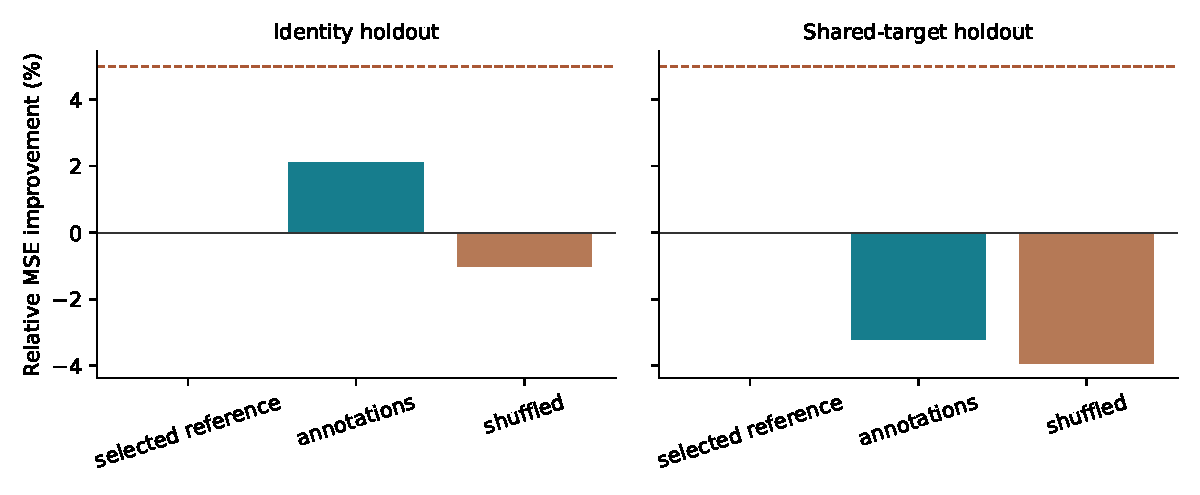
\includegraphics[width=.82\linewidth]{evidence/identity_results.pdf}\caption{Publisher annotations fail both identity and shared-target development gates; the dashed line marks the registered 5\% screen.}\end{figure}
A separate primary-metadata audit aligns all 799,317 cell identities with no condition or annotation mismatches, without reading expression outcomes. It recovers one original sample identifier, two replicate labels per line, and 48 line/culture control strata. Original culture labels alias existing assigned plate strata, supplying no independently initiated culture evidence beyond the randomized treatment wells already documented. The count matrix is not refitted. Pair responses, multiple sealed states, biological covariance for empirical power, and independent risk evaluation remain absent. Recovery of metadata nomenclature does not create fresh confirmation.
